% !TeX encoding = UTF-8
\documentclass[aspectratio=169]{beamer}
\useoutertheme[progressbar=frametitle]{metropolis}
\useinnertheme{metropolis}
\definecolor{nabgray}{rgb}{0.6,0.59,0.61}
\usecolortheme[named=nabgray]{structure}
% Code syntax highlighter
\usepackage{minted}
\usepackage{tikz}
\usepackage[utf8]{inputenc}
\usepackage[spanish]{babel}
\usepackage{fontspec}
\setmonofont{JetBrains Mono}
\setmainfont{Roboto}
\setsansfont{Roboto}

\usepackage{smartdiagram}
\usepackage{qtree}
\usepackage{verbatim}
\usepackage{svg}
\usepackage{graphicx}
\usepackage{color}

\definecolor{lightgray}{rgb}{0.95, 0.95, 0.95}
\definecolor{darkgray}{rgb}{0.4, 0.4, 0.4}
%\definecolor{purple}{rgb}{0.65, 0.12, 0.82}
\definecolor{editorGray}{rgb}{0.95, 0.95, 0.95}
\definecolor{editorOcher}{rgb}{1, 0.5, 0} % #FF7F00 -> rgb(239, 169, 0)
\definecolor{editorGreen}{rgb}{0, 0.5, 0} % #007C00 -> rgb(0, 124, 0)
\definecolor{orange}{rgb}{1,0.45,0.13}
\definecolor{olive}{rgb}{0.17,0.59,0.20}
\definecolor{brown}{rgb}{0.69,0.31,0.31}
\definecolor{purple}{rgb}{0.38,0.18,0.81}
\definecolor{lightblue}{rgb}{0.1,0.57,0.7}
\definecolor{lightred}{rgb}{1,0.4,0.5}
\usepackage{upquote}
\usepackage{listings}
\lstset{language=java,
	basicstyle=\footnotesize\ttfamily,
	keywordstyle=\footnotesize\color{blue}\ttfamily,
	escapeinside={<@}{@>}
}
\lstset{language=XML,
	basicstyle=\footnotesize\ttfamily,
	keywordstyle=\footnotesize\color{blue}\ttfamily,
	escapeinside={<@}{@>}
}

\usebackgroundtemplate%
{%
	
\includegraphics[width=\paperwidth]{Images/Contenido}%
}


\title{Gestión de cargas de trabajo con Eclipse JKube}
\author{Víctor Orozco}
\institute{GuateJUG}
\date{}

\begin{document}





{
    \usebackgroundtemplate{
\includegraphics[width=\paperwidth]{Images/portada}}
    \setbeamercolor{frametitle}{fg=red}
    \usebeamercolor[fg]{normal text}
    \frame{\titlepage}
}


\begin{frame}{Kubernetes}
\Large Entendamos las cargas de trabajo
\end{frame}

\begin{frame}{Kubernetes - Crear la carga}

\begin{itemize}
\item Programar y depurar la aplicación
\item Empacar la aplicación (.war/.jar)
\item Escribir el Dockerfile
\item Crear la imagen OCI
\end{itemize}

\end{frame}

\begin{frame}{Kubernetes - El caminó a hacia Kubernetes}
\begin{itemize}
\item Imagen OCI
\item Contenedor (Pod)
\item ReplicaSet
\item Variable
\item Mountpoint
\item Secret
\item Deployment
\end{itemize}
\end{frame}


\begin{frame}{Kubernetes - El camino desde Kubernetes al mundo}
\begin{itemize}
\item SVC
\item Ingress
\item Healthcheck
\item Metrics
\end{itemize}
\end{frame}


\begin{frame}{Descriptor YAML}
	\begin{columns}[T] % contents are top vertically aligned
		
		\begin{column}[T]{4cm} % alternative top-align that's better for graphics
        Ventajas
		\begin{enumerate}
			\item Fácil de leer
			\item Soportado en cualquier editor
            \item Común en DevOps -e.g. Github Action, Bitbucket Pipelines-
		\end{enumerate}
		\end{column}
		\begin{column}[T]{6cm} % each column can also be its own environment
			\begin{figure}
            \centering
            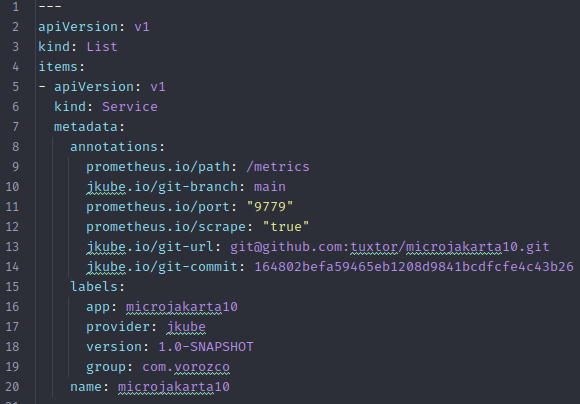
\includegraphics[width=\linewidth]{Images/yaml}
            \end{figure}
			
		\end{column}
	\end{columns}
\end{frame}

\begin{frame}{Helm}

		\begin{enumerate}
			\item + Aplicaciones como paquetes (Charts) 
			\item + Parametrizable
			\item - Proyecto independiente
            \item - Crear un chart es complejo
		\end{enumerate}
        
        \begin{figure}
        \centering
        
\includegraphics[width=0.6\linewidth]{Images/helm}
        \end{figure}


\end{frame}


\begin{frame}{Kustomize}

		\begin{enumerate}
			\item + Plantillas en stack
			\item + Versión independiente o nativa
            \item + Genera (al vuelo) descriptores a partir de bases
			\item - Sigue siendo YAML
            \item - Aun así es una tarea adicional
		\end{enumerate}
        
\begin{figure}
\centering
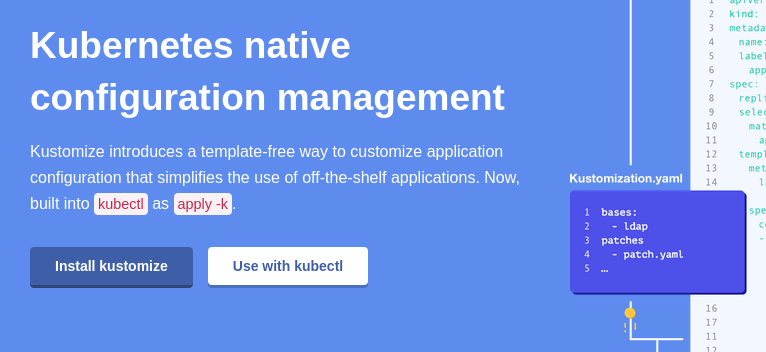
\includegraphics[width=0.6\linewidth]{Images/kustomize}
\end{figure}


\end{frame}




{
	\usebackgroundtemplate{
\includegraphics[width=\paperwidth]{Images/separador}}
	\setbeamercolor{normal text}{fg=white}
	\setbeamercolor{frametitle}{fg=red}
	\usebeamercolor[fg]{normal text}
	\section{Eclipse JKube}
}


\begin{frame}[fragile]{Maven}

           	\begin{itemize}
           		\item Software Project Management
           		\item Compilación y \textbf{generación} de código
           		\item Reportes
           		\item Documentación
                \item Estándar de facto
           	\end{itemize}

\end{frame}

\begin{frame}[fragile]{Single source of truth?}
    \begin{columns}
        \begin{column}{0.5\textwidth}
        Maven
           	\begin{itemize}
           		\item Nombre de artefactos
           		\item Perfiles y entornos
           		\item Ejecución de tareas (mvn)
           	\end{itemize}
        \end{column}
        \begin{column}{0.5\textwidth}  %%<--- here
        Kubernetes descriptor
          \begin{itemize}
    		\item Nombre de contenedores OCI
       		\item Perfiles basados en plantillas
       		\item Ejecución de tareas (Kubectl)
        	\end{itemize}
        \end{column}
    \end{columns}
\end{frame}




\begin{frame}{Eclipse JKube}
	\begin{columns}[T] % contents are top vertically aligned
		
		\begin{column}[T]{4cm} % alternative top-align that's better for graphics
		\begin{enumerate}
			\item Colección de plugins Maven y Gradle
			\item Construcción: Docker, JIB o S2I
            \item Despliegue: Kubernetes y/o Openshift
		\end{enumerate}
		\end{column}
		\begin{column}[T]{6cm} % each column can also be its own environment
\begin{figure}
\centering

\includegraphics[width=0.7\linewidth]{Images/jkube}
\end{figure}
			
		\end{column}
	\end{columns}
\end{frame}

\begin{frame}{Eclipse JKube - Configuración}
	\begin{columns}[T] % contents are top vertically aligned
		
		\begin{column}[T]{4cm} % alternative top-align that's better for graphics
		\begin{enumerate}
			\item Zero
			\item Inline (XML)
            \item External (Plantillas)
		\end{enumerate}
		\end{column}
		\begin{column}[T]{6cm} % each column can also be its own environment
\begin{figure}
\centering

\includegraphics[width=0.7\linewidth]{Images/jkube}
\end{figure}
			
		\end{column}
	\end{columns}
\end{frame}

\begin{frame}[fragile]{Eclipse JKube}
Zero (Spring Boot, Vert.x, Wildfly, Quarkus, Open Liberty, Micronaut)
\begin{lstlisting}[language=XML]
<plugin>
    <groupId>org.eclipse.jkube</groupId>
    <artifactId>kubernetes-maven-plugin</artifactId>
    <version>1.9.1</version>
</plugin>
\end{lstlisting}

\end{frame}

\begin{frame}[fragile]{Eclipse JKube}
Personalizado con propiedades
\begin{lstlisting}[language=XML]
<maven.compiler.release>17</maven.compiler.release>
<project.build.sourceEncoding>UTF-8</project.build.sourceEncoding>
<failOnMissingWebXml>false</failOnMissingWebXml>
<version.wildlfy>27.0.0.Beta1</version.wildlfy>
<version.wildfly.datasources.galleon-pack>3.0.0.Beta1</version.wildfly.datasources.galleon-pack>
<version.testcontainers>1.17.5</version.testcontainers>
<version>1.10.1</version>
<jkube.generator.name>iad.ocir.io/idemd9jasawg/microjakarta10:%l</jkube.generator.name>
\end{lstlisting}

\end{frame}



\begin{frame}[fragile]{Eclipse JKube}
Ajustado con plantillas

\begin{figure}
\centering
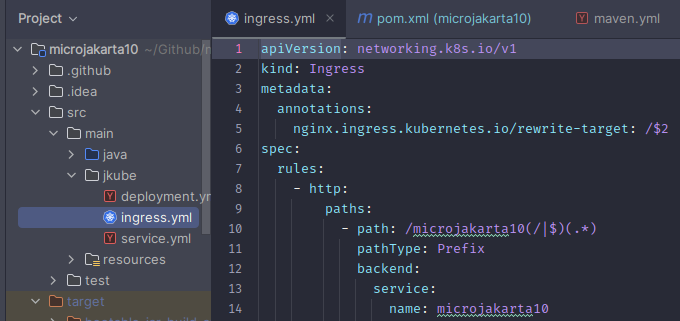
\includegraphics[width=0.7\linewidth]{Images/plantillas}

\end{figure}


\end{frame}

\begin{frame}[fragile]{Eclipse JKube}
Generación de contenedor OCI
\begin{lstlisting}[language=bash]
mvn clean verify k8s:build
\end{lstlisting}

Generación de descriptor 
\begin{lstlisting}[language=bash]
mvn k8s:resource
\end{lstlisting}
\begin{verbatim}
(target/classes/META-INF/jkube/kubernetes.yml)
\end{verbatim}
\end{frame}

\begin{frame}[fragile]{Eclipse JKube}
Despliegue
\begin{lstlisting}[language=bash]
mvn k8s:apply
\end{lstlisting}

Eliminación
\begin{lstlisting}[language=bash]
mvn k8s:undeploy
\end{lstlisting}

Logs
\begin{lstlisting}[language=bash]
mvn k8s:log
\end{lstlisting}

Depuración remota
\begin{lstlisting}[language=bash]
mvn k8s:debug
\end{lstlisting}
\end{frame}

\begin{frame}[fragile]{Eclipse JKube}
Lo amo por
\begin{itemize}
\item Unificación de gestión de proyecto
\item Maven profiles
\item CI/CD
\item Autoconfiguración
\item Reducción de errores
\end{itemize}

Características útiles
\begin{itemize}
\item Desarrollo remoto (k8s:remote-dev)
\item Despliegue continuo en desarrollo (k8s:watch)
\item Helm como alternativa (k8s:debug)
\end{itemize}
\end{frame}

\begin{frame}{Víctor Orozco}
    \begin{columns}[T] % contents are top vertically aligned

        \begin{column}[T]{4cm} % alternative top-align that's better for graphics
            \begin{figure}
                \centering
                
\includegraphics[width=\linewidth]{Images/logos}
            \end{figure}
        \end{column}
        \begin{column}[T]{6cm} % each column can also be its own environment
            \begin{itemize}
                \item me@vorozco.com
                \item \href{https://twitter.com/tuxtor}{@tuxtor}
                \item \href{https://vorozco.com}{http://vorozco.com}
                \item \href{https://tuxtor.shekalug.org}{http://tuxtor.shekalug.org}
            \end{itemize}
            \begin{center}
                
\includegraphics[width=0.1\linewidth]{Images/cclogo}
                \\
                This work is licensed under Creative Commons Attribution-NonCommercial-ShareAlike 3.0 Guatemala (CC BY-NC-SA 3.0 GT).
            \end{center}
        \end{column}
    \end{columns}
\end{frame}



\end{document}
